\documentclass{standalone}
\usepackage{pgfplots}
\pgfplotsset{compat=1.13}

\begin{document}

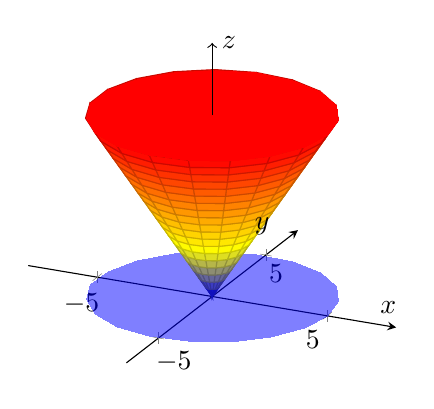
\begin{tikzpicture}
    \begin{axis}[
            axis lines=center,
            hide z axis,
            xlabel={$x$}, ylabel={$y$}, zlabel={$z$},
            domain=0:5,
            y domain=0:2*pi,
            xmin=-8, xmax=8,
            ymin=-8, ymax=8,  zmin=0.0, zmax=7,
            samples=20]
        \addplot3 [surf,z buffer=sort, shader=interp, opacity=0.5] ({x*cos(deg(y))},{x*sin(deg(y))},{0});
        \addplot3 [surf,z buffer=sort] ({x*cos(deg(y))},{x*sin(deg(y))},{x});
        \addplot3 [surf,z buffer=sort, shader=interp, opacity=1] ({x*cos(deg(y))},{x*sin(deg(y))},{5});
        \draw[->, thin] (axis cs:0,0,5) -- (axis cs:0,0,7)  node[anchor=west]{\(z\)};
    \end{axis}
\end{tikzpicture}

\end{document}